\chapter{Angriffe}
\label{chap:attacks}

Betrachtet man nun die unter Kapitel \ref{chap:threads} aufgezeigten Bedrohungen, wundert es nicht, dass es eine Vielzahl von Angriffsvektoren gibt. Um die Möglichkeiten potenzieller Angreifer und damit die möglichen Mitigationsverfahren besser verstehen zu können werden nachfolgend die gängigsten Angriffe auf DNS beschrieben. Dabei wird hier spezieller Fokus auf Client-relevante Gefahren gelegt. Angriffe die weder Vertraulichkeit, noch Integrität oder Verfügbarkeit des Clients gefährden werden nicht behandelt.

\section{DNS Sniffing}
\label{sec:attacks-dnssniffing}
% Sniffing / Spoofing zusammenlegen?

Als Sniffing Angriffe werden alle Arten von Angriffen bezeichnet die es ermöglichen Nachrichten zwischen mindestens 2 Parteien zu beobachten, mitzulesen und/oder mitzuhören\cite{CAPEC157}. In Hinblick auf DNS hat dies eine spezielle Bedeutung da es, aufgrund des fehlenden Schutz der Vertraulichkeit, ermöglicht, alle Informationen der Anfragen und Antworten einzusehen. Somit ist das Kommunikationsverhalten der Opfergeräte leicht nachzuvollziehen, was zum Beispiel den Recon-Schritt der Cyber-Kill-Chain (siehe \ref{sec:dnssecurity}) erheblich erleichtert. Das Aufzeichnen des DNS-Verkehrs lässt außerdem umfangreiche Schlussfolgerungen auf das Kommunikationsverhalten des Opfers zu. Darüber hinaus kann so auch die Transaktions-ID zusammen mit dem Ausgangsport erfahren werden, was die Voraussetzung für eine Spoofing-Attacke (siehe \ref{sec:attacks-dnsspoofing}) darstellt. 

\section{DNS Spoofing}
\label{sec:attacks-dnsspoofing}

Nach CAPEC werden Spoofing Angriffe, auch \textit{Identity Spoofing} genannt, über die Aktion des \"zielgerichteden Glaubhaftmachen einer gefälschten Identität" definiert. Es ist einem Angreifer dadurch möglich, dem Opfer Informationen mitzuteilen, die von diesem als glaubwürdig und richtig eingestuft werden. Im Fall von DNS spricht man von DNS Spoofing, was dieses simple Konzept auf einfache art ausnützt.
Das DNS Netzwerkprotokoll verlässt sich beim prüfen der Authentizität der Antworten nun einerseits auf das Transportprotokoll (meistens UDP) und eine 16-bit Transaktions-ID (TXID) \cite{rfc1035}. Gelingt es einem Angreifer nun sowohl das ausgehende Port, als auch die TXID in Erfahrung zu bringen, ist es einfach möglich eine gefälschte, glaubwürdige Antwort zu generieren (siehe Abb. \ref{img:dnsspoofing}). Kommt diese nun vor der echten Antwort beim Client an oder wird sogar vom Angreifer ganz abgefangen, kann dem Opfer jede beliebige Antwort glaubhaft gemacht werden.

\begin{figure}[htbp]
    \centering
    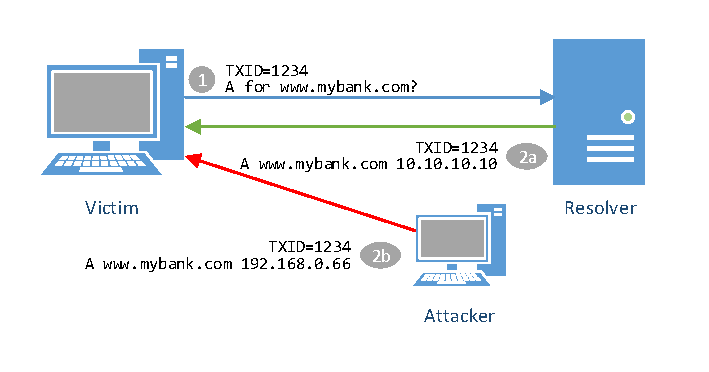
\includegraphics[width=0.7\textwidth]{DNS_Spoofing}
    \caption{}
    \label{img:dnsspoofing}
\end{figure}


\subsection{DNS Cache Poisoning}

DNS Spoofings ermöglicht den DNS-Cache eines Zielrechners aktiv zu Manipulieren. Angriffe die bewusst Einträge in Caches von Opfern verändern werden allgemein als \textit{Cache Poisoning}-Attacken bezeichnet \cite{CAPEC141}. \textit{DNS Cache Poisoning} bietet somit die Möglichkeit, gezielt gefälschte Einträge in die Caches von Servern einzubringen\cite{CAPEC142}. Dies ermöglicht es einem Angreifer Verbindungen zu bestimmten Zieldomänen bewusst umzuleiten oder stillzulegen. Wie in Abb. \ref{img:dnscachepoisoning} zu sehen ist, wird für eine erfolgreiche Attacke kein Zugriff auf das Netzwerk des Opfers benötigt. Nachdem der Client die Anfrage an seinen Resolver abgesetzt hat (1), wird die Adresse über den rekursive Auflöseprozess ermittelt (2,3,4,5a). Sendet ein Angreifer nun Antworten mit der gefälschten Absendeadresse des authoritativen Nameservers an den Resolver (5b), wird diese vom Resolver akzeptiert, sollte sie die richtige TXID enthalten und vor der echten Antwort ankommen. Aufgrund der geringen Entropie der TXID (16-bit) ist das simple Erraten dieser ID zwar mühsam aber durchführbar \cite{Son2010}.      

\begin{figure}[htbp]
    \centering
    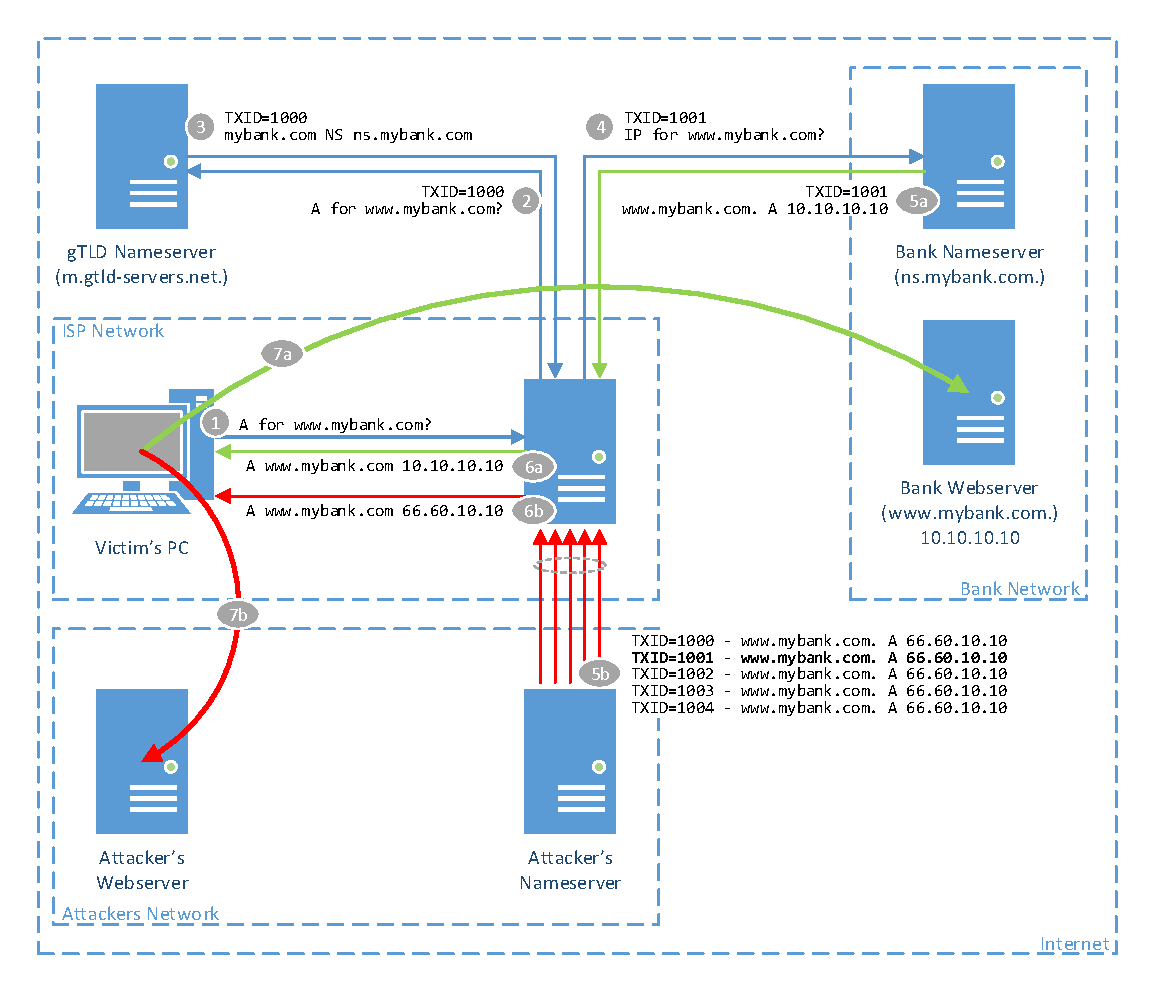
\includegraphics[width=\textwidth]{DNS_CachePoisoning}
    \caption{}
    \label{img:dnscachepoisoning}
\end{figure}

\subsection{Kaminsky Angriff}

Eine viel gefährlichere Variante der Attacke ist 2008 vom amerikanischen Sicherheitsexperte Dan Kaminsky entwickelt worden\cite{Son2010}. In Abbildung \ref{img:dnskaminsky} wird gezeigt, wie es möglich ist, den Aufwand und die notwendige Zeit des Cache Poisonings massiv zu reduzieren. Dafür wird die Tatsache ausgenützt, dass die meisten Ziel-Resolver auch vom Angreifer erreichbar sein. Wird nun eine Anfrage zum Auflösen einer nicht existenten Unterdomäne der Zieldomäne an den Resolver gestellt (1) beginnt dieser mit der normalen Auflösung (2,3,4,5a). Da die Domäne nicht vorhanden ist, kann sie auch nicht in den Cache aufgenommen werden. Unterdessen sendet der Angreifer, wie im normalen Cache Poisoning auch, gefälschte Antworten an den Resolver. Diese enthalten jedoch neben der Auskunft, dass die Domäne nicht existiert einen zusätzlichen Eintrag der den Resolver über einen neuen Nameserver Eintrag informiert. Dieser gefälschter Eintrag enthält jedoch die Adresse eines Nameservers unter der kontrolle des Angreifers. Gelingt nun das einbringen der falschen Antwort, würde der Resolver ab diesem Zeitpunkt alle Anfragen an die Ziel-Domäne zum Nameserver des Angreifers weiterleiten. Dies stellt die effektive Übernahme der gesamten Domäne dar.
Der Vorteil dieses Angriffs besteht in seiner beliebigen Wiederholbarkeit, da der eigentliche Eintrag nicht gecacht wird. Da der Auflöseprozess außerdem bewusst vom Angreifer initiiert wird, ist das korrekte Timing einfacher, die Attacke dadurch zuverlässiger.

\begin{figure}[htbp]
    \centering
    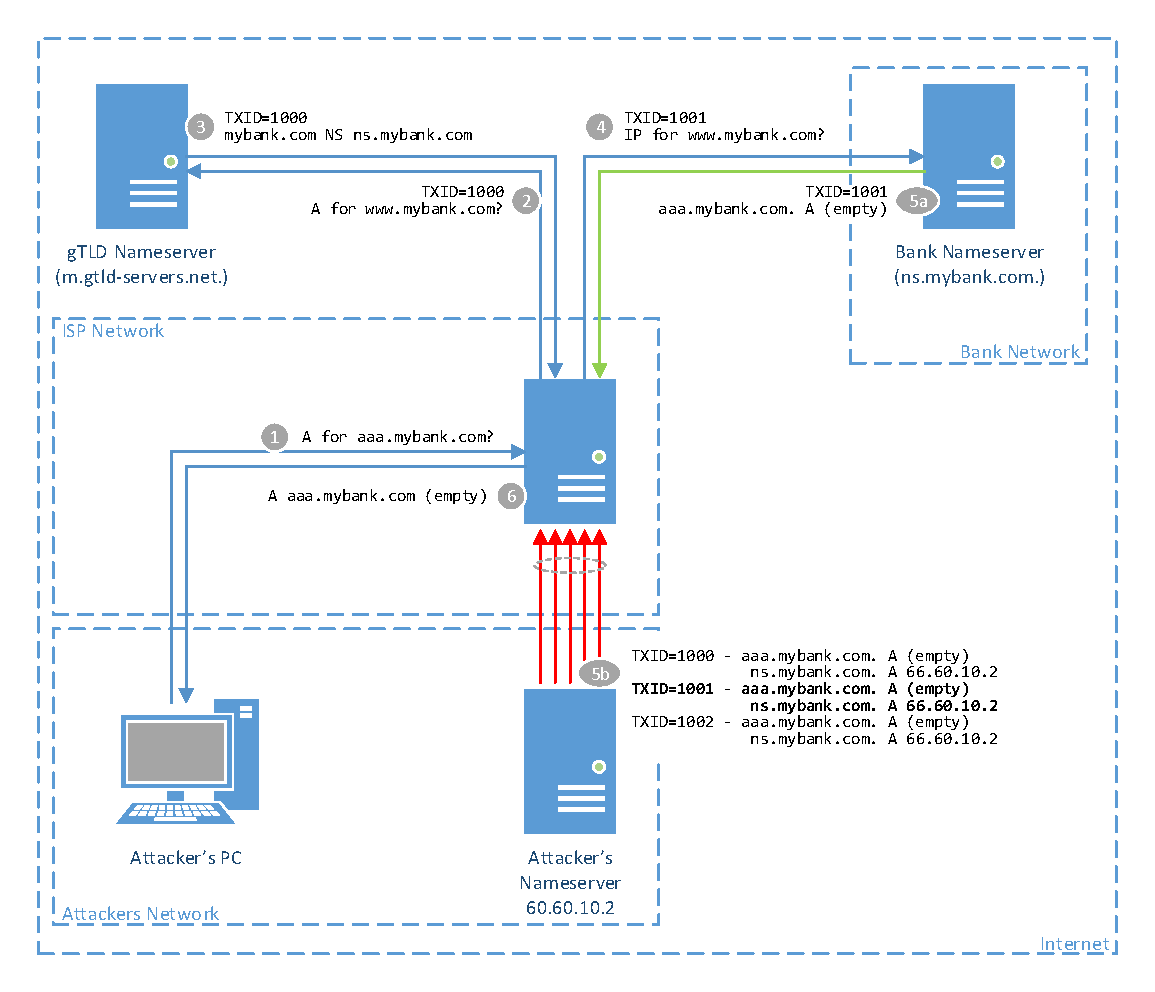
\includegraphics[width=\textwidth]{DNS_Kaminsky}
    \caption{}
    \label{img:dnskaminsky}
\end{figure}

\section{Man-In-The-Middle Angriff}

Wie viele ältere Protokolle ist auch DNS von einer starken anfälligkeit gegen sogenannte Man-in-the-Middle (MITM) Attacken betroffen. Dies Art des Angriffs zeichnet sich durch den Umstand aus, dass sich der Angreifer unbemerkt zwischen zwei Kommunikationsteilnehmer Positionieren kann \cite{CAPEC94}. Aufgrund seiner vermittelnden Position ist er somit in kompletter Kontrolle der Kommunikation ist kann diese nach belieben manipulieren. Da dieser Angriff derartig mächtig ist, bieten sich jedoch effektivere Wege um die Kontrolle über die Ziele auszuweiten. Die genauen Angriffswege und Möglichkeiten der Ausnutzung werden von Conti, Dragoni und Lesyk \cite{Conti2016} ausführlich beschrieben und würden den Rahmen dieser Arbeit sprengen.

\section{DNS Rebinding}
\label{sec:attack-dnsrebind}

Eine weniger bekannte Art die Schwachstellen von DNS auszunutzen ist das sogenannte \textit{DNS Rebinding}. Kern des Angriffs besteht in der Tatsache, dass moderne Browser aufwendige Sicherheitsmechanismen haben, um den unerlaubten Zugriff zwischen verschiedenen Websites und Hosts zu unterbinden. Diese als \textit{Access Within Same Origin Policy} genannte Technik verbietet es Scripts einer Webseite auf Inhalte zuzugreifen die nicht unter dem selben Hostnamen erreichbar sind. Es können zwar Ausnahmen definiert werden, da dies jedoch am Ziel passieren muss, besteht dadurch keine Gefahr. Die auszunützende Schwachstelle besteht nun im Fakt, dass DNS-Einträge mit sehr geringer TTL gesetzt werden können. Es wird dadurch möglich die Adresse eines Namens während der Ausführung eines Scripts zu verändern \cite{Jackson2009}. Das ermöglicht den folgenden Ablauf.

\begin{enumerate}
    \item Das Opfer wird vom Angreifer auf eine von ihm kontrolliere Website gelockt. Der Nameserver des Angreifers vergibt für den Eintrag eine sehr geringe TTL.
    \item Der Browser des Opfers führt die Scripts, welches auf der Webseite eingebunden sind aus. Gleichzeitig läuft die TTL des gecachten Eintrags aus was den Resolver zu einer erneuten Auflösung gewegt. Bei dieser wird nun vom Nameserver des Angreifers die Adresse eines Ziels zurückgeliefert.
    \item Nach diesem \textit{Rebinding} des Hostnamen kann das laufende Script über den eigenen Namen auf die Ressourcen der Adresse des Ziels zugreifen. Dies erlaubt den Script Zugriffe auf netzinterne Ressourcen wie Administrationsoberflächen oder ermöglicht das Scannen des LANs. Außerdem wird damit der Browser des Opfers für andere Angriffe, wie Click Fraud oder DoS Attacken, nutzbar.   
\end{enumerate}

Auch wenn es viele Gegenmaßnahmen in aktuellen Browsern gibt und einige der anfälligen Komponenten (Java Applets, Flash, etc.) an Verbreitung verlieren, besteht besonders durch die zunehmende Verbreitung von IoT-Geräten eine akute Bedrohung durch diesen Angriffsweg \cite{Dorsey2018}. 

\section{Denial-Of-Service Angriff}

Denial-Of-Service Attacken (DoS) zielen darauf ab die Nutzung bestimmter Dienstleistungen, Funktionen oder Geräte zu verhindern \cite{BSIG040}. Durch einen solchen Angriff auf den verwendeten Resolver oder relevante, authentitive DNS-Servern können kritischen Unternehmensdienste kurzfristig außer Betrieb genommen werden. Normale Internet-Dienstleistungen weisen heutzutage einen hohen Vernetzungsgrad untereinander auf. Da diese Verbindungen stark von DNS abhängig sind, hat der Ausfall eines einzigen zentralen Dienstes schwerwiegende Auswirkungen auf alle anhängenden Dienste. Dieser Effekt zeigte sich zuletzt 2016 als einer der größten DNS-Anbieter Dyn, inc. von einer DoS-Attacke für mehrere Stunden lahmgelegt wurde \cite{Krebs2016}. DNS ist zwar nicht anfälliger auf DoS als andere zentrale Internet-Services, das Schadensausmaß bei einer erfolgreichen Attacke ist jedoch unvergleichbar hoch. Aus diesem Grund, ist DNS seit Jahren das meist angegriffene Internet-Service weltweit \cite{Alcoy2017}. 

\section{DoS-Amplification Angriff}
\label{sec:attack-dosamp}

Die Nutzbarkeit von DNS als Verstärker (Amplifier) von DoS Attacken ist schon länger bekannt und wurde auch schon früher als Problem erkannt \cite{ICANN2006}. Nach dem Anual Wordwide Infrastructure Security Report 2017 befindet sich DNS als Trägertechnologie von DoS-Attacken auf Platz 1 \cite{Alcoy2017}. Die leichte Ausnutzbarkeit und schlechte Zurückverfolgbarkeit macht DNS neben NTP zu den beliebtesten Verstärkungsmethoden. Wie Anagnostopoulos et al.\cite{Anagnostopoulos2013} und van Rijswijk-Deij et at.\cite{VanRijswijk-Deij2014} zeigen konnte besteht darüber hinaus das Problem, dass DNSSEC die Situation bei steigender Verbreitung weiter verschärft. Mithilfe von DNSSEC konnte ein durchschnittlichen Verstärkungsfaktor von 47,2 erreicht werden, wobei die maximale Verstärkungsrate bei DNS ohne DNSSEC bei 12,8 liegt. Dieser Umstand ist auf die mit DNSSEC eingeführte Erweiterung EDNS0 zurückzuführen, die es ermöglicht Antworten, die größer als die ursprüngliche Grenze von 512 bytes sind, zu empfangen. Es konnte gezeigt werden, dass 90\% der offenen Resolver maximale Packetgrößen von 4k bytes unterstützen, was bei einer Anfragegröße von 40 byte einen maximalen Verstärkungsfaktor von 102,4 zulassen würde. Dies birgt zusammen mit anderen Kritikpunkten ein massives Hemmnis für die Verbreitung von DNSSEC und ist unter anderem ein Grund für die schlechte Verbreitungsrate. Das Kernproblem liegt hier jedoch an dem eingesetztem Transportprotokoll UDP zusammen mit dem Umstand, dass DNS keinerlei Authentifizierung des Clients verlangt. Betrachtet man andere Protokolle mit ähnlichen Bedingungen (z.B. NTP) zeichnet sich ein ähnliches Bild. Der Vorwurf an DNSSEC als Verursacher der DoS-Amplifikation Problematik ist somit kritisch zu betrachten.

\section{BitSquatting}

Eine weiter Angriffsmöglichkeit bietet das sogenannte \textit{BitSquatting}. Bei diesem Angriff werden zufällige Fehler im Speicher von Geräten ohne fehlererkennenden Speichermodulen ausgenützt. Es konnte gezeigt werden, dass es durch solche Fehler zum stellen fehlerhafter Anfragen an potenziell existente Domänen kommen kann\cite{Dinaburg2011}. Dieser Effekt kann nun bewusst ausgenutzt werden indem eine große Anzahl an Domänen registriert werden, deren Name sich nur um ein Bit von viel besichten Domänen unterscheidet (siehe Listing \ref{lst:bitquatting}). Da es dadurch zu falschen Anfragen kommt, gibt es auch keine Möglichkeit sich auf Protokoll- bzw. System-Ebene zu schützen. Die einzige effektive Lösung stellt der Einsatz von \textit{Error-correcting code memory} Hardware dar.  

\begin{lstlisting}[caption={Drei mögliche BitSquatting-Domänen für die Zieldomäne \texttt{amazon.com}}, label={lst:bitquatting}]
amazon.com = 61   6d   61 7a   6f   6e 2e 63 6f 6d
           ... 01101101 ... 01101111 ... 
aeazon.com = 61   65   61 7a   6f   6e 2e 63 6f 6d  
           ... 01100101 ...
                   ^
a-azon.com = 61   e2   61 7a   6f   6e 2e 63 6f 6d 
           ... 00101101 ...
                ^
amazgn.com = 61   6d   61 7a   67   6e 2e 63 6f 6d
                        ... 01100111 ...
                                ^
\end{lstlisting}
